\TOWRITE{ALL}{Proofread 4. Members of the consortium pass 2}

\subsection{Participants}

\eucommentary{Please provide, for each participant, the following (if available):\\
\begin{compactitem}
\item
a description of the legal entity and its main tasks,
with an explanation of how its profile matches the tasks in the proposal;
\item
a curriculum vitae or description of the profile of the persons,
including their gender, who will be primarily responsible for carrying
out the proposed research and/or innovation activities;
%
this includes a description of the profile of the to-be-recruited personnel
\item
a list of up to 5 relevant publications, and/or products, services
(including widely-used datasets or software), or other achievements
relevant to the call content;
\item
a list of up to 5 relevant previous projects or activities, connected
to the subject of this proposal;
\item
a description of any significant infrastructure and/or any major items
of technical equipment, relevant to the proposed work;
\item
any other supporting documents specified in the work programme for this call.
\end{compactitem}}

\begin{sitedescription}{SRL}

Simula is an internationally-leading Norwegian research institute in the key
ICT areas: communication systems, scientific computing and software
engineering. Simula's research areas have been evaluated with the highest
score by international expert panels in several national evaluations.

Dedicated to tackling scientific challenges with long-term impact and of
genuine importance to real life, Simula offers an environment that emphasises
and promotes basic research. This translates into numerous projects funded by
the EU, Norwegian government or regional institutions, that Simula was
involved in. In 2017, it successfully concluded Norwegian Centre of Excellence
for Biomedical Computing and is currently hosting the Centre for
Research-based Innovation, Certus. In addition, Simula is deeply involved in
research education with 35 PhD students, 40 master's students, and 20
postdoctoral fellows supervised annually; and application-driven innovation
and commercialisation, where it owns parts of 16 start-up companies with 110
employees.

The Department for Numerical Analysis and Scientific Computing (SCAN) aims to
develop mathematical methods and scientific tools to reach new understanding
of complex physical processes. It targets fundamental medical and industrial
problems where new insights from mathematical modelling can advance today's
knowledge. The department has hosted a ten-year Norwegian Centre of Excellence
in Biomedical Computing (2007-2017), one of the most prestigious research
environments in Norway, targeting ambitious and groundbreaking research. The
department received top scores in all six evaluations carried out by the
Research Council of Norway and is running a multitude of national and
international research projects, including one ERC Starter Grant project.

\subsubsection*{Curriculum vitae}
% Curriculum of the personnel at this institution

\begin{participant}[type=leadPI,PM=28,gender=male]{Benjamin Ragan-Kelley}
  % PM=YYY:
  % A fair evaluation of the number of months you will be
  % spending on this specific project along the four years.
  % Typical numbers:
  % - full time hired personnel: 48 months
  % - lead PI or proposal coordinator: 8-12 months
  % - PI: 4-5 months
  % - participant: 2-6 months

  % salary=ZZZ:
  % Approximate monthly gross salary (in term of total cost for the
  % employer). This is optional. If you are uncomfortable having this
  % information in a public file, you can alternatively send the
  % information to Eugenia Shadlova, or to your institution
  % leader/manager if he is willing to fill in himself the budget
  % forms on the eu portal.

Benjamin Ragan-Kelley is one of the core maintainers and developers
of the Jupyter and IPython projects, and currently leads the JupyterHub
and BinderHub development teams.
He has been a contributor to these projects since 2006,
prior to the establishment of Jupyter as a separate project from IPython.
He is an expert in all levels of Jupyter development,
especially the aspects of deploying Jupyter-based services,
which is the focus of this proposal.
Benjamin will lead \TheProject.

Beyond Jupyter, Benjamin has contributed widely to open source software,
especially in the scientific Python community.
He is a maintainer of numerous scientific packages
in the conda-forge package management system,
building packages used widely in education and research,
such as PETSc, MPICH, and FEniCS.

Benjamin is a Research Engineer in the department of Scientific Computing and Numerical Analysis
at Simula Research Laboratory in Oslo, Norway,
where his primary responsibility is developing and maintaining the Jupyter software ecosystem,
as well as supporting research scientists in diverse fields,
including biomedical computing.

Prior to his current position at Simula,
Benjamin received his Bachelor's degree \textit{Magne cum Laude} in Engineering Physics in 2007
from Santa Clara University and his PhD in Applied Science and Technology
from the University of California, Berkeley in 2013.
He worked as a postdoctoral fellow at Simula Research Laboratory prior
to becoming a permanent Research Engineer.
He was honored along with the rest of the Jupyter steering council
with the 2017 ACM Software System Award for Jupyter.


\end{participant}

%%% Local Variables:
%%% mode: latex
%%% TeX-master: "../proposal"
%%% End:


\input{CVs/Katarina.Subakova.tex}

\begin{participant}[PM=72, type=R]{Research Engineer x2}

We will hire two postdoctoral-level research engineers to carry out the work
at Simula, under the leadership of and together with Dr. Ragan-Kelley.  The
fellow will have a background in computational science, combined with IPython
and Jupyter Notebook experience, and past experience of software engineering.
An ideal candidate will also have good communication skills and team working
abilities, and in particular interest and skill in the development and
operation of software services to best support this part of the project.

\end{participant}


\subsubsection*{Publications, products, achievements}

\begin{compactenum}
\item 2017 ACM Software System Award for Jupyter
\item M. Bussonier, J. Forde, J. Freeman, B. Granger, T. Head, C. Holdgraf, K.
  Kelley, G. Nalvarte, A. Osheroff, M. Pacer et al. Binder 2.0 - Reproducible,
  interactive, sharable environments for science at scale In Python in Science
  ConferenceProceedings of the 17th Python in Science Conference. Austin,
  Texas: SciPy, 2018.
\item J. Forde, T. Head, C. Holdgraf, Y. Panda, G. Nalvarte, M. Pacer, F.
  Perez, B. Ragan-Kelley and E. Sundell. Reproducible Research Environments
  with Repo2Docker In ICML 2018 Reproducible Machine Learning. ICML, 2018.
\item T. Kluyver, B. Ragan-Kelley, F. Perez, B. Granger, M. Bussonier, J.
  Frederic, K. Kelley, J. Hamrick, J. Grout, S. Corlay et al. Jupyter
  Notebooks: a publishing format for reproducible computational workflows In
  20th International Conference on Electronic Publishing. IOS Press, 2016.

\end{compactenum}

\subsubsection*{Relevant projects or activities}

\begin{compactenum}
\item OpenDreamKit (GA No. 676541) Open Digital Research Environment Toolkit for the Advancement of Mathematics, participant, Work Package lead
\item Jupyter - collaboration with UC Berkeley, Cal Poly, funded by Gordon \&
  Betty Moore Foundation, Alfred P. Sloan Foundation, and Helmsley Trust
\item Binder - collaboration with UC Berkeley, funded by Gordon \& Betty Moore
  Foundation
\end{compactenum}

\subsubsection*{Significant infrastructure}

The fully owned Simula subsidiary Simula Innovation handles pre-commercial
innovation projects, creation and follow-up of company spin-offs, and general
support for entrepreneurs.

\end{sitedescription}



%KEY-MORE-TODOS


%%% Local Variables:
%%% mode: latex
%%% TeX-master: "../proposal"
%%% End:

%  LocalWords:  sitedescription Simula Simula commercialisation Certus subsubsection Logg
%  LocalWords:  Mardal Funke Rognes Sci Comput Langtangen FEniCS Aln ae lgaard vspace
%  LocalWords:  TOWRITE emphasises organised

\clearpage
\begin{sitedescription}{CDS}

\begin{center}
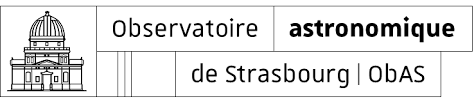
\includegraphics[height=3cm]{Participants/Logos/OAS.png}
\end{center}

The Observatoire Astronomique de Strasbourg (ObAS) is a Joint Research Unit
(UMR7550) of the CNRS and of the Université de Strasbourg. ObAS hosts the 
Centre de Données astronomiques de Strasbourg (Strasbourg astronomical Data 
Centre CDS, http://cds.unistra.fr). Since its creation in 1972, the CDS has 
been providing reference services which are widely used by the world-wide 
astronomical community with more than 1 million queries/day on average in 
2017. The CDS is labelled as a Research Infrastructure in the French national
Research Infrastructure Roadmap. Since 2006 CDS has been the coordinator,
on behalf of the CNRS, of all the projects funded by the European Commission
to support the implementation of European Virtual Observatory. 

% PIC:
% see: http://ec.europa.eu/research/participants/portal/desktop/en/organisations/
%
% See ../proposal.tex, section Members of the Consortium for a
% complete description of what should go there

\subsubsection*{Curriculum vitae}

% Curriculum of the personnel at this institution. This includes
% to-be-hired people for which there is a tentative candidate.

%\input{CVs/First.Last.tex}
%\input{CVs/First.Last.tex}

\input{CVs/Mark.Allen.tex}
\input{CVs/Thomas.Boch.tex}
\input{CVs/Sebastien.Derriere.tex}

\begin{participant}[type=R,PM=12,salary=4200]{Software Engineer}
    We intend to hire a software engineer for 12 months during the project to be be supervised at CDS to work on developments defined in Task \taskref{applications}{astro}. We aim to hire someone in the period of months 12-24. 
\end{participant}

% For other to-be-hired person, please include here something like:
% \begin{participant}[type=res,PM=3,salary=5900]{NN}
%  <a _short_ description of the qualifications of whom you want to hire>
% \end{participant}

\subsubsection*{Publications, products, achievements}

\begin{compactenum}
  \item F. Genova, M. G. Allen, C. Arviset, A. Lawrence, F. Pasian, E. Solano, J. Wambsganss, Euro-VO - Coordination of Virtual Observatory activities in Europe, Astronomy and Computing, 2015, Volume 11, p. 181-189
  \item F. Genova et. al 2017, Building a Disciplinary, World-Wide Data Infrastructure. Data Science Journal, 16: 16, pp. 1-13, DOI: https://doi.org/10.5334/dsj-2017-016
  \item P. Fernique, M. G Allen, T. Boch, A. Oberto, F-X. Pineau, D. Durand, C. Bot, L. Cambresy, S. Derriere, F. Bonnarel, F. Genova, Hierarchical Progressive Surveys - Multi-resolution HEALPix data structures for astronomical images, catalogues and 3-dimensional data cubes.  2015, A \& A, 578, A114 
  \item M. Baumann, T.Boch, New Python developments to access CDS services, Proceedings of The Astronomical Data Analysis Software and Systems conference 2018.
\end{compactenum}

\subsubsection*{Relevant projects or activities}

\begin{compactenum}
  \item ESCAPE (EC funded project, 2019-2023, \#824064, INFRAEOSC-0402018)
  \item ASTERICS (EC funded project, 2015-2019, \#653477, Research and Innovation Action)
  \item AENEAS (EC funded project,  2017-2020, \#731016, Research and Innovation Action)
  \item CoSADIE - Collaborative and Sustainable Astronomical Data Infrastructure for Europe (EC funded project \#312559, 2012-2015, CSA)
  \item RDA Europe - the European plug-in to the Research Data Alliance (RDA) (EC funded project \#632756, 2014-2016, CSA)
\end{compactenum}

\subsubsection*{Significant infrastructure}

CDS is data centre for reference astronomy data. CDS runs physical infrastructure for 1Petabyte. Connected to French national network RENATER. Computing power for X-Match and generation of all-sky survey data. Currently running prototype notebook servers.


\end{sitedescription}
%%% Local Variables:
%%% mode: latex
%%% TeX-master: "../pro%%% End:

\clearpage
\begin{sitedescription}{EP}

\begin{center}

\includegraphics[height=3cm]{Participants/Logos/EP.png}
\end{center}

\'Ecole Polytechnique (l'X), is the leading member of Grandes \'Ecoles in France
for science and technology according to all French rankings last year, ranked
2nd best small university in the world by Times Higher Education in 2018, and
16th best European university by QS World University Rankings in 2018. With
fewer than 3000 Bachelor, Masters, and PhD students enrolled at any time, the
institution has produced 4 Fields Medalists, 4 Nobel prize winners, and 3 French
presidents, ranking it 6th worldwide in terms of number of Nobel prize
recipients. L'X is composed of 22 laboratories supporting research in physics,
engineering, mathematics, biology, and chemistry (among others) and is connected
to several French national research institutions such as CNRS, CEA, and INRIA.
L'X prides itself on promoting multidisciplinary research through collaboration
between its many labs and with external, national and international partners and
a strong connection with industry and start-up.

The Mathematics department at Ecole polytechnique has started a reform of their
various teaching offer based on Jupyter. Many courses from the
Bachelor program, Engineering school, and the Master program have
already begun relying on a strong use of Jupyter notebooks /
JupyterHub\footnote{\url{http://www.cmap.polytechnique.fr/~massot/Personal_web_page_of_Marc_Massot/MAP551}} and this will continue with a strong support of the Dean of
undergraduate studies and of graduate studies. In addition, several software and
research engineers in applied mathematics have been recruited and
participate, together with a system engineer, to this effort in order to help in terms of
building an infrastructure dedicated to Jupyter.
This infrastructure together with support from the head of the Ecole polytechnique,
fosters the dissemination into various other
departments (Physics, Mechanical Engineering, Biology...), where some
Jupyter-based courses are already starting.
A community is emerging, notably through the strong engagement of
students in the computer science club of \'Ecole polytechnique (Binet R\'eseau).

\subsubsection*{Curriculum vitae}
% Curriculum of the personnel at this institution. This includes
% to-be-hired people for which there is a tentative candidate.

\begin{participant}[type=leadPI,PM=8,gender=male]{Loic Gouarin}

  Loic Gouarin is Research Engineer in scientific computing at CMAP (Centre de
  Mathématiques Appliquées) which is a Joint Research Unit
  (UMR7641) of the CNRS and \'Ecole polytechnique. He works on several
  scientific computing open-source projects in different fields such as
  Lattice-Boltzmann methods, Stokes solvers for fluid particles interaction,
  adaptive mesh refinement, ...

  He is also director of the ``GdR Calcul'' where his role is to animate the
  scientific and high performance computing community in France, in particular
  by organising conferences, meetings, and seminars. In this context, he
  organises himself 3 to 4 training and development workshops per year, and
  promotes the use of Python and c++ for teaching and research in France.
  
  For several years, he has been very involved in promoting the Jupyter project
  and its use for teaching and research in the French community. He is one of
  the core developers of xeus-cling and he is working on the possibility of
  easily deploying a JupyterHub or BinderHub on academic clouds. He also
  believes that reproducible research is an essential part of promoting new
  computation codes, new numerical methods, ... introduced in related
  publications and therefore he uses Jupyter as a first approach to achieve this.
  
  \end{participant}
  
  %%% Local Variables:
  %%% mode: latex
  %%% TeX-master: "../proposal"
  %%% End:
  
\begin{participant}[type=R,PM=4,gender=male]{David Delavennat}

    David Delavennat is Research Engineer in scientific infrastructures at CMLS
    (Centre de Mathématiques Laurent Schwartz) which is a Joint Research Unit
    (UMR7640) of the CNRS and \'Ecole polytechnique. He
    works on several french scientific infrastructures projects using
    microservices, virtualization, container and cloud technologies.

    He is coordinator of ARGOS, the Paris-South business network targeted to the
    academic System and Network Administrators. He animates this community,
    organising conferences and meetings He represents ARGOS at RESINFO, the
    french business network of regional SNA business networks. In this context,
    he participate each year to the organization of National Teaching Actions.

    For several years, he has been very involved in promoting the DevOps
    paradigm and Continuous Integration for deploying production infrastructures
    on academic Openstack and Kubernetes environment for the French Mathematical
    community. He is working on simplifying the deployment of a JupyterHub or
    BinderHub onto academic PaaS and Iaas. He also believes that reproducible
    infrastructures is an essential part of reproducible science.

\end{participant}
\input{CVs/Marc.Massot.tex}
\begin{participant}[type=R,PM=2,gender=male]{Laurent Series}

    Laurent Series is Research Engineer in scientific computing at CMAP (Centre 
    de Mathématiques Appliquées) which is a Joint Research Unit
    (UMR7641) of the CNRS and \'Ecole polytechnique. He works on several
    scientific computing open-source projects in different fields like
    finite element method for solid mechanics, multiresolution for 
    reaction-diffusion equations modeling multi-scale reaction wave ...
  
    He was technical responsible of Computing Center (M\'esocentre) of Ecole
    CentraleSup\'elec from 2009 to 2018. In this context, he organises and 
    participates in the user support team (assistance in porting codes, 
    parallelization, vectorisation, optimisation). Since his arrival at \'Ecole 
    Polytechnique, he is involved in the process of creation of a new Computing 
    Center.
    
    For several years, he has been very involved in promoting the Jupyter project
    by writing Jupyter notebooks for course (such as "Dynamical systems for the 
    modeling and simulation of multi-scale reacting media" MAP551) and by promoting, 
    among researchers, its use to share their work. He is also involved with the 
    direction of \'Ecole polytechnique for the project of building an infrastructure 
    for Jupyter at the level of the school, for its use in both research and teaching.
  
\end{participant}

% For other to-be-hired person, please include here something like:
\begin{participant}[type=R,PM=18,salary=5500]{DevOps Engineer}
  We intend to hire a DevOps engineer for 18 months during the project to be supervised at \'Ecole polytechnique to work on developments defined in Tasks \taskref{core}{jh-bh-conv} and \taskref{eosc}{jh-bh-deployment}.
\end{participant}

\begin{participant}[type=R,PM=18,salary=5500]{Software Engineer}
  We intend to hire a DevOps engineer for 18 months during the project to be supervised at \'Ecole polytechnique to work on developments defined in Task \taskref{ecosystem}{teaching-tools}.
\end{participant}

\subsubsection*{Publications, products, achievements}

\begin{compactenum}
\item D. Delavennat, L. Gouarin, G. Philippon, \emph{Deploying JupyterHub with Kubernetes on OpenStack} \newline
\url{https://blog.jupyter.org/how-to-deploy-jupyterhub-with-kubernetes-on-openstack-f8f6120d4b1}
\item JupyterDay at \'Ecole polytechnique in 2018 \newline
\url{http://www.cmap.polytechnique.fr/~massot/Personal_web_page_of_Marc_Massot/JupyterX.html}
\item L. Gouarin, \emph{C++ course using xeus-cling} \newline
\url{https://github.com/gouarin/cours_cpp_moderne}
\item M.Massot, L. Series, \emph{Systèmes dynamiques pour la modélisation et la simulation des "milieux réactifs" multi-échelles} \newline
\url{http://www.cmap.polytechnique.fr/~massot/Personal_web_page_of_Marc_Massot/MAP551}
\end{compactenum}

\subsubsection*{Relevant projects or activities}

\begin{compactenum}
\item Through a previous position at Paris Sud, Loïc Gouarin is a
  participant of OpenDreamKit (GA No. 676541) Open Digital Research
  Environment Toolkit for the Advancement of Mathematics.
\end{compactenum}

\subsubsection*{Significant infrastructure}

\site{EP} has strongly contributed to the deployment of JupyterHub on
\site{UPSUD}'s local OpenStack based cloud infrastructure
\software{Cloud@VD}. \site{EP} invested last year in the purchase of 100 cores for this infrastructure in order to study how to deploy JupyterHub and BinderHub and start to offer to researchers and students this kind of service.
In 2019, \site{EP} will have its own OpenShift cloud infrastructure with 200-300 cores dedicated to teaching with Jupyter.

\end{sitedescription}
%%% Local Variables:
%%% mode: latex
%%% TeX-master: "../proposal"
%%% End:

\clearpage
\begin{sitedescription}{EGI}


The EGI Foundation (also known as Stichting EGI and abbreviated as EGI.eu) 
is a not-for-profit foundation established under the Dutch law to coordinate 
the EGI Federation (abbreviated as EGI), an international collaboration that 
federates the digital capabilities, resources and expertise of national and 
international research communities in Europe and worldwide. 
The main goal is to empower researchers from all disciplines to collaborate 
and to carry out data- and compute-intensive science and innovation. 
The EGI Foundation coordinates areas such as overseeing infrastructure operations, 
user community support, contact with technology providers, strategy and policy 
development, flagship events and dissemination of news and achievements. 
As part of its mandate, the EGI Foundation actively represents the EGI federation 
at European level with policy makers and funding agencies, it provides expert 
advice to shape policies and funding programs and also support the implementation 
of the policy priorities. 
The EGI Foundation holds certifications in both ISO/IEC 9000 “Quality Management” 
and ISO/IEC 20000 “IT Service Management”. 

% PIC:
% see: http://ec.europa.eu/research/participants/portal/desktop/en/organisations/
%
% See ../proposal.tex, section Members of the Consortium for a
% complete description of what should go there

\subsubsection*{Curriculum vitae}
\TODO{AK - rules say "CV or description of the profile of the persons"
  can we name it "Track record" instead of CV?}

% Curriculum of the personnel at this institution. This includes
% to-be-hired people for which there is a tentative candidate.

%\input{CVs/First.Last.tex}
\begin{participant}[type=leadPI,PM=,gender=male]{Gergely Sipos}

    Gergely Sipos works as Technical Outreach Manager for EGI.eu. 
    He coordinates user engagement and supports activities in the EGI community, 
    supporting scientific communities in exploiting EGI services to push scientific 
    boundaries. 

    He holds MSc and PhD in computer science with specialisation in management, 
    from the University of Miskolc (Hungary).

\end{participant}


% For other to-be-hired person, please include here something like:
% \begin{participant}[type=res,PM=3,salary=5900]{NN}
%  <a _short_ description of the qualifications of whom you want to hire>
% \end{participant}

\subsubsection*{Publications, products, achievements}

\begin{compactenum}
\item David, M.; Borges, G.; Pina, J. et al., "Validation of Grid Middleware for the European Grid Infrastructure", (2014) DOI: 10.1007/s10723-014-9301-z 
\item Ferrari, T.; Gaido, L., "Resources and Services of the EGEE Production Infrastructure", Journal of Grid Computing, June 2011, Volume 9, Issue 2, pp 119-133, DOI: 10.1007/s10723-011-9184-1, June 2011. 
\item Matti Heikkurinen, Sandra Cohen, Fotis Karagiannis, Kashif Iqbal, Sergio Andreozzi, Michele Michelotto, "Answering the Cost Assessment Scaling Challenge: Modelling the Annual Cost of European Computing Services for Research", Journal of Grid Computing, May 2014, DOI:10.1007/s10723-014-9302-y 
\item Sy Holsinger, Sergio Andreozzi, "EGI: Implementing service management in a large-scale e-Infrastructure", Proceedings of the IEEE Network Operations and Management Symposium (NOMS) Conference, 2014, Krakow, Poland, DOI: 10.1109/NOMS.2014.6838371
\item Sergio Andreozzi, Sy Holsinger, Damir Marinovic, Steven Newhouse, "EGI: an Open e-Infrastructure Ecosystem for the Digital European Research Area", Proceedings of eChallenges e-2012 Conference, Lisbon, Portugal, ISBN: 978-1-905824-35-91 
\item Ohmann, C.; Canham, S.; Danielyan, E.; Robertshaw, S.; Legr\'e, Y.; Clivio, L. \& Demotes, J., "Cloud computing and clinical trials: report from an ECRIN workshop", Commentary Trials, Springer, December 2015, 16:318, DOI: /10.1186/s13063-015-0835-6 \newline
\item Wallom, D.C.H.; Turilli, M., Drescher, M.; Scardaci, D. \& Newhouse, S., "Federating Infrastructure as a Service Cloud Computing Systems to Creates a Uniform EInfrastructure for Research", IEEE 11th International Conference on e-Science 2015, DOI:10.1109/eScience.2015.51
\item Cloud, Fernandez, E.; Sipos, G.; Scardaci, D.; Wallom, D.C.H. \& Chen, Y., "The user support programme and the training infrastructure of the EGI Federated Cloud", International Conference on High Performance Computing \& Simulation (HPCS) 2015, DOI: 10.1109/HPCSim.2015.7237016 
\item Sergio Andreozzi, Owen Appleton, Sara Coelho, Tiziana Ferrari, Sy Holsinger, Yannick Legr\'e, "Open Science Commons", Jan 2015, http://go.egi.eu/oscwp
\item Kimmo Koski, Kristiina Hormia-Poutanen, Prof. Mike Chatzopoulos, Yannick Legré, Bob Day, "European Open Science Cloud for Research", Oct 2015, https://zenodo.org/record/32915
\end{compactenum}

\subsubsection*{Relevant projects or activities}

\begin{compactenum}
\item EGI-Engage: Engaging the Research Community towards an Open Science Commons
\item EGI-InSPIRE: Integrated Sustainable Pan-European Infrastructure for Researchers in Europe, Project Coordinator, RI-261323
\item AARC (from May 2015)
\item BioMedBridges (Nr 284209)
\item BioVeL (Nr 283359)
\item Civic Epistemologies: Development of a Roadmap for Citizen Researchers in the Digital Culture, RI-632694
\item CloudWATCH: A European cloud observatory supporting cloud policies, standard profiles and services, RI-610994
\item DCH-RP (Nr 312274)
\item e-Fiscal: Financial Study for Sustainable Computing e-Infrastructures, RI-283449
\item EDISON: Creating the Data Science Profession (Nr 675419)
\item ENVRI (Nr 283465)
\item ENVRIplus (Nr 654182)
\item ER-Flow (Nr 312579)
\item eScienceTalk: Supporting grid and high performance computing reporting across Europe, Project Coordinator, RI-260733
\item FedSM: Implementing Service Management in Federated e-Infrastructures, RI-312851
\item Helix Nebula Science Cloud Project, the (from January 2016)
\item HelixNebula: Big science teams up with big business, RI-312301
\item INDIGO-DataCloud (from May 2015)
\end{compactenum}

\subsubsection*{Significant infrastructure}

EGI Infrastructure: The EGI Foundation coordinates the delivery of the EGI Infrastructure that brings together more than 300 data centres worldwide and also includes the largest community cloud federation in Europe with 21 cloud providers across 12 European countries offering IaaS cloud and storage services. The Infrastructure includes a Jupyter Hub that is open for researchers on the scalable EGI IaaS cloud.

\end{sitedescription}
%%% Local Variables:
%%% mode: latex
%%% TeX-master: "../proposal"
%%% End:

\clearpage
\begin{sitedescription}{XFEL}
  \label{sitedescription:euxfel}

% PIC:
% see: http://ec.europa.eu/research/participants/portal/desktop/en/orga

% See ../proposal.tex, section Members of the Consortium for a
% complete description of what should go there

  European X-Ray Free-Electron Laser Facility GmbH is a limited
  liability company under German law. At present, 12 countries are
  participating in the project: Denmark, France, Germany, Hungary,
  Italy, Poland, Russia, Slovakia, Spain, Sweden, Switzerland, and the
  United Kingdom.  The company is in charge of the operation and
  construction of the European XFEL, a 3.4 km long X-ray free-electron
  laser facility extending from Hamburg to the neighbouring town of
  Schenefeld in the German federal state of Schleswig-Holstein. Civil
  construction started in early 2009, and the user operation in
  September 2017. With its repetition rate of 27,000 pulses per second
  and a peak brilliance a billion times higher than that of the best
  synchrotron X-ray radiation sources, the European XFEL will allow
  the investigation of still open scientific problems in a variety of
  disciplines (physics, structural biology, chemistry, planetary
  science, study of matter under extreme conditions and many others).

  European XFEL has a data policy in place \cite{datapolicy-euxfel}
  which opens up facility data for open access after an embargo period
  of 3 years.
\subsubsection*{Curriculum vitae}

% Curriculum of the personnel at this institution
%
\input{CVs/Hans.Fangohr.tex}
\input{CVs/Sandor.Brockhauser.tex}
\begin{participant}[type=PI,PM=1,gender=male]{Krzysztof Wrona}
  % type is one of:
  % - leadPI: leader of the participating institution
  % - PI: Principal Investigator
  % - R: researcher?
  % Who is the coordinator is specified elsewhere

  % PM=YYY:
  % A fair evaluation of the number of months you will be
  % spending on this specific project along the four years.
  % Typical numbers:
  % - full time hired personnel: 48 months
  % - lead PI or proposal coordinator: 8-12 months
  % - PI: 4-5 months
  % - participant: 2-6 months

  % salary=ZZZ:
  % Approximate monthly gross salary (in term of total cost for the
  % employer). This is optional. If you are uncomfortable having this
  % information in a public file, you can alternatively send the
  % information to Eugenia Shadlova, or to your institution
  % leader/manager if he is willing to fill in himself the budget
  % forms on the eu portal.

  % The above information is used to fill in various tables in the
  % proposal file, and to evaluate the cost of the project for the
  % institutions.

  % You may remove all those comments.

  % About half a page of free text; for whatever it's worth, you may see
  % Nicolas.Thiery.tex for an example.



  \medskip Krzysztof Wrona has a background in computer physics. As
  the group leader of IT and Data Management at European XFEL, he is
  in charge of the management of scientific data in the frame of the
  user program of the European XFEL facility. He has more than 15
  years of experience in data storage, processing, and in general IT
  issues.
\end{participant}

%%% Local Variables:
%%% mode: latex
%%% TeX-master: "../proposal"
%%% End:

\input{CVs/Thomas.Kluyver.tex}
%


\begin{participant}[PM=68, type=R]{Research Engineer x2}

We will hire two postdoctoral-level research software engineers (for 68 person
months in total) to carry out the required work for this projet at
European XFEL. They will work under supervision of Hans Fangohr, with
support from Sandor Brockhauser and Krzysztof Wrona for particular
aspects. The employees will either have a scientific background and
significant software engineering expertise, or an education in
computer science and an aptitude to work with scientists on
computational science and data science problems.
\end{participant}

\subsubsection*{Publications, products, achievements}

\begin{compactenum}
\item H.Fangohr, Python for Computational Science and Engineering
  (2018) DOI: 10.5281/zenodo.1411868 \newline
  https://github.com/fangohr/introduction-to-python-for-computational-science-and-engineering
\item H.Fangohr et al., “Data Analysis support in Karabo at European
  XFEL”, Proceedings of International Conference on Accelerator and
  Large Experimental Physics Control Systems 2017, ISBN 978-3-95450-
  193-9, Data Analytics, Barcelona, Spain, TUCPA01 (2017) DOI: 10.18429/JACoW-ICALEPCS2017-TUCPA01
\item H.Fangohr.
\emph{A Comparison of \software{C}, \Matlab and \Python as Teaching Languages in Engineering}
Lecture Notes on Computational Science \textbf{3039}, 1210-1217 (2004)
\item T. Kluyver, B. Ragan-Kelley, F. Perez, B. Granger, M. Bussonier, J. Frederic, K. Kelley, J. Hamrick, J. Grout, S. Corlay et al. Jupyter
\emph{Notebooks: a publishing format for reproducible computational workflows} In 20th International Conference on Electronic Publishing. IOS Press, 2016.
\end{compactenum}

\subsubsection*{Relevant projects or activities}

\begin{compactenum}
\item OpenDreamKit (GA No. 676541) Open Digital Research Environment
  Toolkit for the Advancement of Mathematics, participant
\item EOSCpilot (GA No. 739563) The European Open Science Cloud for
  Research Pilot Project, participant
\item PaNOSC (GA No. 823852) Photon and Neutron Open Science Cloud,
  participant
\item CALIPSOplus (GA No. 730872) Convenient Access to Light Sources
  Open to Innovation, Science and to the World, participant
\item ATTRACT (GA No. 777222) breAkThrough innovaTion pRogrAmme for a
  pan-European Detection and Imaging eCosysTem, participant

\end{compactenum}




\end{sitedescription}



%KEY-MORE-TODOS



%%% Local Variables:
%%% mode: latex
%%% TeX-master: "../proposal"
%%% End:

%  LocalWords:  sitedescription Programme organisations programmes Centres subsubsection
%  LocalWords:  micromagnetic Nmag Fischbacher Franchin Bordignon Fangohr emph textbf
%  LocalWords:  Multiphysics summarised Iridis TFlops Modelling

\clearpage
\begin{sitedescription}{INSERM}

Inserm, the French National Institute of Health \& Medical Research is the only
public sector research institution in France exclusively dedicated to human
health. Under the dual aegis of the Ministries of Health and Research, Inserm
has a budget of 900 M euros and employs 15,000 scientists, engineers and
technicians all with one shared objective, namely to promote health - by
advancing knowledge about living organisms and their diseases, developing
innovative treatment modalities and conducting research on public health.

Inserm is represented within the BOSSEE consortium through the Cancer Research
Centre of Toulouse (CRCT) and Inserm’s Computing Department (D\'epartement du
Système D’Information, DSI).

CRCT gathers academic, scientific, medical, clinical, technological and
pharmaceutical research on cancer on a 220-hectares site next to Toulouse,
France. Its missions are to improve fundamental knowledge on all aspects of
cancer biology and to provide patients with rapid access to innovative and
individualized treatments. On these premises, CRCT comprises 21 teams
affiliated to Inserm, the University of Toulouse and the CNRS (National Centre
for Scientific Research). Team 15 of CRCT led by M. Bardi\`es aggregates
Medical Physics resources available in Toulouse around a common research theme:
the optimization of radiotherapy through the development of innovative
dosimetric approaches at various scales (cell, tissue, patient).

Inserm's IT department (DSI) defines and coordinates IT and information systems
aspects across the whole institution. It designs and operates Inserm's
information system to support research activities of the institute, and
provides counselling and support to research units on information technologies.
It also plays a strong role in coordinating IT security and risk management
policies for the French health science community.

% PIC:
% see: http://ec.europa.eu/research/participants/portal/desktop/en/organisations/
%
% See ../proposal.tex, section Members of the Consortium for a
% complete description of what should go there

\subsubsection*{Curriculum vitae}
% Curriculum of the personnel at this institution. This includes
% to-be-hired people for which there is a tentative candidate.
\begin{participant}[type=leadPI,PM=3,gender=male]{Manuel Bardi\`es}
  % type is one of:
  % - leadPI: leader of the participating institution
  % - PI: Principal Investigator
  % - R: researcher?
  % Who is the coordinator is specified elsewhere

  % PM=YYY:
  % A fair evaluation of the number of months you will be
  % spending on this specific project along the four years.
  % Typical numbers:
  % - full time hired personnel: 48 months
  % - lead PI or proposal coordinator: 8-12 months
  % - PI: 4-5 months
  % - participant: 2-6 months

  % salary=ZZZ:
  % Approximate monthly gross salary (in term of total cost for the
  % employer). This is optional. If you are uncomfortable having this
  % information in a public file, you can alternatively send the
  % information to Eugenia Shadlova, or to your institution
  % leader/manager if he is willing to fill in himself the budget
  % forms on the eu portal.

  % The above information is used to fill in various tables in the
  % proposal file, and to evaluate the cost of the project for the
  % institutions.

  % You may remove all those comments.

  % About half a page of free text; for whatever it's worth, you may see
  % Nicolas.Thiery.tex for an example.

  Manuel Bardi\`es, PhD, obtained his doctorate on radiopharmaceutical
  dosimetry from Paul Sabatier University (Toulouse III) in 1991. He has been
  developing his research in radiopharmaceutical dosimetry within INSERM
  (National Institute of Health and Medical Research), since 1992, in Nantes
  then in Toulouse (2011) within the Cancer Research Centre of Toulouse (CRCT).
  He is the responsible of CRCT Team 15 entitled "Multi- resolution dosimetry
  for radiotherapy optimization".
  
  Dr. Bardi\`es has been appointed to several international positions. He was
  one of the founders of the EANM Dosimetry Committee (member from 2001 to
  2013, chair 2009-2011). He also chaired of EFOMP Science Committee
  (2014-2016).
  
  Dr. Bardi\`es is also involved in education and is currently member of the
  Board of the European School for Medical Physics Expert (ESMPE) and member of
  the European School of Multimodality Imaging and Therapy (ESMIT).
  
  The team led by Manuel Bardi\`es in Toulouse (CRCT Team 15) is primarily
  involved in radiopharmaceutical dosimetry, at various scales (cell, tissue,
  organs). This requires the ability to assess radiopharmaceutical
  pharmacokinetics in vivo, through quantitative SPECT or PET small-animal
  imaging. An important part of research activity is related to Monte Carlo
  modelling of radiation transport through biological structures of interest,
  in order to give account of energy deposition within tumour targets - or
  critical non-tumour tissues/organs. The objective is to improve molecular
  radiotherapy by allowing patient-specific treatments, as an important
  application of personalized medicine.

\end{participant}

%%% Local Variables:
%%% mode: latex
%%% TeX-master: "../proposal"
%%% End:

\input{CVs/Maxime.Chauvin.tex}
\begin{participant}[type=PI,PM=6,gender=female]{Isabelle Perseil}
  % type is one of:
  % - leadPI: leader of the participating institution
  % - PI: Principal Investigator
  % - R: researcher?
  % Who is the coordinator is specified elsewhere

  % PM=YYY:
  % A fair evaluation of the number of months you will be
  % spending on this specific project along the four years.
  % Typical numbers:
  % - full time hired personnel: 48 months
  % - lead PI or proposal coordinator: 8-12 months
  % - PI: 4-5 months
  % - participant: 2-6 months

  % salary=ZZZ:
  % Approximate monthly gross salary (in term of total cost for the
  % employer). This is optional. If you are uncomfortable having this
  % information in a public file, you can alternatively send the
  % information to Eugenia Shadlova, or to your institution
  % leader/manager if he is willing to fill in himself the budget
  % forms on the eu portal.

  % The above information is used to fill in various tables in the
  % proposal file, and to evaluate the cost of the project for the
  % institutions.

  % You may remove all those comments.

  % About half a page of free text; for whatever it's worth, you may see
  % Nicolas.Thiery.tex for an example.

  Isabelle Perseil, PhD, is the Head of the Computational Science Coordination
  and e-infrastructures of Inserm. Dr. Perseil manages a group of 3 experts
  which provides the best practices in software engineering, Data Management,
  Big data, deep learning, HPC, Grids, Cloud Computing, parallel computing to
  300 research units (1200 research teams).
  
  The Computational Science Coordination is working with 13 regional
  administrations and 23 regional Mesocenters to pool the computational
  resources (grids and HPC) and train more than 1000 engineers and researchers
  to HPC (OpenMP, MPI and now ORWL) and Big data (MapReduce, Hadoop, Spark,
  Flink, Storm).

\end{participant}

%%% Local Variables:
%%% mode: latex
%%% TeX-master: "../proposal"
%%% End:

\input{CVs/Gilles.Mathieu.tex}

% For other to-be-hired person, please include here something like:
% \begin{participant}[type=res,PM=3,salary=5900]{NN}
%  <a _short_ description of the qualifications of whom you want to hire>
% \end{participant}

\subsubsection*{Publications, products, achievements}
\begin{compactenum}
\item A. Albeyatti et al. “Towards a European health research and innovation
  cloud (HRIC)”. In: 2019 accepted in Genome Medicine.
\item M. Chauvin et al. “OpenDose: Generating reference data for Nuclear
  Medicine dosimetry”. In: European Journal of Nuclear Medicine and Molecular
  Imaging 44.S2 (Sept. 2017), pp. 119--956. DOI: 10.1007/s00259-017-3822-1.
\item D. Salas et al. “Resource-Centered Distributed Processing of Large
  Histopathology Images”. In: 2016 IEEE Intl Conference on Computational
  Science and Engineering (CSE) and IEEE Intl Conference on Embedded and
  Ubiquitous Computing (EUC) and 15th Intl Symposium on Distributed Computing
  and Applications for Business Engineering (DCABES). Aug. 2016, pp. 367--370.
  DOI: 10.1109/CSE-EUC-DCABES.2016.210.
\item S. Marcatili et al. “Model-based versus specific dosimetry in diagnostic
  context: Comparison of three dosimetric approaches”. In: Medical Physics 42.3
  (2015), pp. 1288--1296. DOI: 10.1118/1.4907957.
\item D. Sarrut et al. “A review of the use and potential of the GATE Monte
  Carlo simulation code for radiation therapy and dosimetry applications”. In:
  Medical Physics 41.6 Part1 (2014), p. 064301. DOI: 10.1118/1.4871617.
\item I. Perseil et al. “An Efficient Modeling and Execution Framework for
  Complex Systems Development”. In: 2011 16th IEEE International Conference on
  Engineering of Complex Computer Systems. Apr. 2011, pp. 317--331. DOI:
  10.1109/ICECCS.2011.38.
\item  A. Divoli et al. “Effect of Patient Morphology on Dosimetric
  Calculations for Internal Irradiation as Assessed by Comparisons of Monte
  Carlo Versus Conventional Methodologies”. In: Journal of Nuclear Medicine
  50.2 (2009), pp. 316--323. DOI: 10.2967/jnumed.108.056705.
\item I. Perseil and L. Pautet. “Foundations of a new software engineering
  method for real-time systems”. In: Innovations in Systems and Software
  Engineering 4.3 (Oct. 2008), pp. 195--202. ISSN: 1614-5054. DOI:
  10.1007/s11334-008-0067-y
\end{compactenum}

\subsubsection*{Relevant projects or activities}
Inserm is the leading academic biomedical research institution in Europe with
more than 13,000 publications a year; and second in the world (behind the
American National Institutes of Health).

Inserm has 24 international cooperation agreements, 33 associated European
laboratories (AELs) and associated international laboratories (AILs), and 183
Horizon 2020 contracts since 2014 - of which 45 were signed in 2017. 67 ERC
winners have been hosted at Inserm since 2012, 13 of whom in 2017.  Inserm is
involved in many ESFRIs:
\begin{compactenum}
\item ERINHA2 (H2020)
\item ERINHA (FP7)
\item ADOPT BBMRI-ERIC (H2020)
\item BioMedBridges (FP7)
\item MRTdosimetry EMPIR (H2020)
\item MetroMRT (REG)
\end{compactenum}
Inserm is also one of the funding partners of the French NGI, integrated within
EGI.

\subsubsection*{Significant infrastructure}
Inserm has more than 350 research units spread across France and
internationally. These are supported by 13 Regional Commissions for local
oversight. Scientific activities are organized around 9 “Inserm Thematic
Institutes”, corresponding to the main fields of biomedical and health
research.

\end{sitedescription}
%%% Local Variables:
%%% mode: latex
%%% TeX-master: "../proposal"
%%% End:

\clearpage
\begin{sitedescription}{QS}

\begin{center}

\includegraphics[height=3cm]{Participants/Logos/QuantStack.png}
\end{center}

\par QuantStack was founded in 2016 by a team of developers and maintainers of key packages of the open-source scientific computing stack. QuantStack provides support and custom development services in the Jupyter and Scientific Python ecosystems. Clients and partners of QuantStack range from financial software companies to robotics startups and public research institutions. The team comprises several core developers of Jupyter subprojects and authors of popular scientific computing and visualization software used in both academic and industrial contexts.

\par Beyond Project Jupyter, projects developed at QuantStack include data visualization packages for Jupyter such as bqplot, ipyvolume, ipyleaflet, and ipysheet, as well as Jupyter language kernels such as xeus-cling and xeus-python, and JupyterLab extensions like te draw.io and sidecar. QuantStack is also behind the development of the xtensor framework, a high-level array computing library and C++ dataframe.

\subsubsection*{Curriculum vitae of the investigators}

\input{CVs/Sylvain.Corlay.tex}
\input{CVs/Johan.Mabille.tex}
\input{CVs/Martin.Renou.tex}
\input{CVs/Wolf.Vollprecht.tex}

% For other to-be-hired person, please include here something like:
\begin{participant}[type=R,PM=41,salary=7000]{Software Engineer} %% Salary: standard SME cost
  We will hire a software engineer with experience working in large open-source
  projects. They will benefit from the mentoring of the other Jupyter contributors
  of the QuantStack team.
\end{participant}

\subsubsection*{Publications, products, achievements}

\begin{compactenum}

\item QuantStack developers participate in the continuous development of \emph{Project Jupyter}. The team is especially active in the area of interactive widgets, as well as JupyterLab and the Jupyter Server.

\item QuantStack is the main driving force behind the \emph{xtensor} project, a C++ tensor expression system for high-performance computing. Xtensor comes along with language bindings for Python, R, and Julia, as well as interfaces to BLAS, FFTW, and means to input and output a large number of standard file formats.

\item QuantStack also develops the \emph{xeus} project, a framework for creating Jupyter language kernels. Xeus is used as a foundation for the C++ Jupyter kernel "xeus-cling", built upon the Cling C++ interpreter from CERN. Xeus was also adopted in Kitware's \emph{Slicer} medical imaging software for its Jupyter integration.

\item The QuantStack team includes the authors and maintainers of some of the most popular Jupyter interactive widgets packages, including \emph{bqplot}, a 2-D interactive plotting system, \emph{ipyvolume}, a 3-D volume rendering package, \emph{ipyleaflet}, a maps visualization toolkit.

\item QuantStack contributes extensively to the \emph{conda-forge} project, a community-maintained collection of packages for scientific computing. Nearly a hundred "recipes" for conda-forge are maintained by QuantStack.

\item QuantStack developers are also behind the \emph{vaex} data decimation engine for interactive visualization of large datasets.

\end{compactenum}

\subsubsection*{Relevant projects or activities}

\par Beyond open-source scientific computing development, QuantStack promotes scientific open source software development through the organization of events and by volunteering in non-profit organizations promoting the ecosystem.

\begin{compactenum}

\item QuantStack team members co-organize the regular \emph{PyData Paris Meetup}, a free event series taking place every two to three months. After a year, the group counts over two thousand members in Paris.

\item We also support the \emph{NumFOCUS Fondation} as volunteers as a member of the team is a member of the board of directors of the foundation.

\end{compactenum}

% \subsubsection*{Significant infrastructure}

\end{sitedescription}

%%% Local Variables:
%%% mode: latex
%%% TeX-master: "../proposal"
%%% End:

\clearpage
\begin{sitedescription}{UIO} \label{desc:UIO}

The University of Oslo (UiO) is Norway's oldest institution for research and higher education, with 28,000 students and 6,000 employees. UiO has 8 faculties, 2 museums and several centres. In addition, UiO has 10 Norwegian Centres of Excellence,  is ranked as the world's 62nd university, and has had 5 Nobel prize laureates. UiO aims to become an international hub for the research-based integration of computing into science education and has financed a university-wide hosting service for Jupyter notebooks through JupyterHub  to introduce a computational aspect to all curriculum programs in all science disciplines from bachelor to postdoctoral studies.

The University of Oslo is a Silver Partner to \href{https://carpentries.org}{The Carpentries}, an international successful community driven project with Instructors, Trainers, Maintainers, helpers, and supporters who share a mission to teach foundational computational and data science skills to researchers.

The Department of Geosciences of the Faculty of Mathematics and Natural Sciences is the broadest geoscience research-based teaching environment in Norway, and covers a wide range of disciplines from deep mantle processes to atmospheric sciences. It is organised in five sections and an administrative unit and supports two main strategic research initiatives:

- Land-Atmosphere Interactions in Cold Environments (\href{https://www.mn.uio.no/geo/english/research/groups/latice/}{LATICE})

- Interface Dynamics in Geophysical Flows (\href{https://www.mn.uio.no/geo/english/research/groups/earthflows/}{EarthFlows})


 The geosciences department has several large research projects financed by \href{https://www.forskningsradet.no/en/Home_page/1177315753906}{The Research Council of Norway}, EU and Norwegian companies.

 The University of Oslo aims to manage research data according to international standards, such as the \href{https://www.uio.no/for-ansatte/arbeidsstotte/fa/forskningsdata/fair-data/index.html}{FAIR principles}\footnote{Findable, Accessible, Interoperable and Reusable}, and thereby support the development of a global research community in which research data is widely shared.
 Since November 2017, UiO’s policy follows the "open as standard" principle in respect of access to research data \cite{datapolicy-uio}.

\subsubsection*{Curriculum vitae}

% Curriculum of the personnel at this institution. This includes
% to-be-hired people for which there is a tentative candidate.

\begin{participant}[type=R,PM=24,gender=female]{Anne Fouilloux}
  % type is one of:
  % - leadPI: leader of the participating institution
  % - PI: Principal Investigator
  % - R: researcher?
  % Who is the coordinator is specified elsewhere

  % PM=YYY:
  % A fair evaluation of the number of months you will be
  % spending on this specific project along the four years.
  % Typical numbers:
  % - full time hired personnel: 48 months
  % - lead PI or proposal coordinator: 8-12 months
  % - PI: 4-5 months
  % - participant: 2-6 months

  % salary=ZZZ:
  % Approximate monthly gross salary (in term of total cost for the
  % employer). This is optional. If you are uncomfortable having this
  % information in a public file, you can alternatively send the
  % information to Eugenia Shadlova, or to your institution
  % leader/manager if he is willing to fill in himself the budget
  % forms on the eu portal.

  % The above information is used to fill in various tables in the
  % proposal file, and to evaluate the cost of the project for the
  % institutions.

  % You may remove all those comments.

  % About half a page of free text; for whatever it's worth, you may see
  % Nicolas.Thiery.tex for an example.

  \medskip PhD, is a highly experienced Research Software Engineer dedicated to supporting
  researchers towards the adoption of Open Science best practices.

  With a solid background in Computer Sciences, she worked in various application fields, including environmental sciences, Intelligent Transport Systems, High-Performance computing, bio-informatics, meteorology and Geosciences.

  She is currently working in the IT group of the department of Geosciences at the University of Oslo\footnote{\url{https://www.mn.uio.no/geo/english}} and for the Nordic e-Infrastructure Collaboration (NeIC\footnote{\url{https://neic.no}}) where she is involved on the NICEST\footnote{Nordic Collaboration on e-Infrastructures for Earth System Modeling, \url{https://neic.no/nicest/}} and CodeRefinery\footnote{Training and e-Infrastructure for Research Software Development, \url{https://coderefinery.org/}} projects. 

   Since 2015, Anne Fouilloux has been very active with The Carpentries\footnote{\url{https://carpentries.org}}, a diverse and global community of volunteers and she teaches foundational coding and data science skills to students and young researchers. She is a certified Carpentries instructor\footnote{\url{https://carpentries.org/instructors/}}, instructor trainer\footnote{\url{https://carpentries.org/trainers/}} and maintainer\footnote{\url{https://carpentries.org/maintainers/}}. She has volunteered to help build CarpentryCon 2020\footnote{\url{http://www.carpentrycon.org/}} a biannual conference for members of the global Carpentries community and people with similar interests. 

  She is a member of the core team of the Carpentries@UiO\footnote{\url{https://www.uio.no/english/for-employees/support/research/research-data/training/carpentry/}} and is leading the studyGroup@UiO\footnote{\url{https://uio-carpentry.github.io/studyGroup/}} where students and researchers at the University of Oslo are committed to sharing skills, experiences, and ideas around open science, open source, code, and community in research.
\end{participant}

%%% Local Variables:
%%% mode: latex
%%% TeX-master: "../proposal"
%%% End:


%\input{CVs/First.Last.tex}
%\input{CVs/First.Last.tex}
%\input{CVs/First.Last.tex}

% For other to-be-hired person, please include here something like:
% \begin{participant}[type=res,PM=3,salary=5900]{NN}
%  <a _short_ description of the qualifications of whom you want to hire>
% \end{participant}

\subsubsection*{Publications, products, achievements}

\begin{compactenum}
\item \href{https://annefou.github.io/jupyter_publish/}{Publication ready scientific reports and presentations with Jupyter notebooks}, Anne Fouilloux, Research Bazaar 2019, \href{https://zenodo.org/badge/latestdoi/163517733}{DOI 10.5281/zenodo.2548936}

\item \href{https://annefou.github.io/jupyter_dashboards/}{Reproducible Research with Interactive Jupyter Dashboards}, 2018, Ana Costa Conrado, Gladys Nalvarte, Benjamin Ragan-Kelley and Anne Fouilloux, Research Bazaar 2018, \href{https://zenodo.org/badge/latestdoi/114125668}{DOI 10.5281/zenodo.1168721}

\item \href{https://annefou.github.io/metos_python/}{Working with Spatio-temporal data in Python}, 2017, Anne Fouilloux, \href{https://zenodo.org/badge/latestdoi/96184802}{DOI 10.5281/zenodo.1165281}
\end{compactenum}

\subsubsection*{Relevant projects or activities}

\begin{compactenum}
\item \href{https://coderefinery.org}{CodeRefinery} \label{desc:coderefinery} (2016-2021): 


The goal of this project is to provide students and researchers with infrastructure and training in the necessary tools and techniques to create sustainable, modular, reusable, and reproducible software.
This is a project within the Nordic e-Infrastructure Collaboration (\href{https://neic.no}{NeIC}), an organisational unit under \href{https://www.nordforsk.org/en}{NordForsk}.
NeIC is a Platinium Partner to \href{https://carpentries.org}{The Carpentries}.

The result of this project is a set of software development e-infrastructure solutions, coupled with necessary technical expertise and extensive training and on-boarding activities, training material and best practices guides which together form a Nordic platform for research groups and institutes to develop a better collaboration on software and thereby to catalyze reproducible research and collaboration.
\newline
CodeRefinery training material is licensed under \href{https://creativecommons.org/licenses/by-sa/4.0/}{CC BY-SA 4.0} and code examples are \href{https://opensource.org/}{OSI}-approved \href{https://opensource.org/licenses/mit-license.html}{MIT license}.

The University of Olso is a CodeRefinery partner and will ensure the complementarity of the two projects thus avoiding potential fragmentation. \TheProject will benefit from all this experience as well as the estbalished network in the Nordic Countries and beyond to fully realize the potential of \TheProject EOSC services. 
\newline


\item Nordic Collaboration on e-Infrastructures for Earth System Modeling (\href{https://neic.no/nicest}{NICEST}, 2017-2019) \label{desc:nicest}:

This project aims at networking, intensifying existing collaboration, and facilitating 
joint work on very specific topics helping, for example, building up knowledge and
competency, and harmonising certain procedures concerning e-Infrastructure topics.

\item \href{https://uiohive.github.io/Hive/}{UiOHive} (2018-2019) \label{desc:uiohive}: 

UiOHive provides a vital and novel competence at the Union of Internet of Things (IoT), Microcontroller / Hardware development, Artificial Intelligence (AI) and Machine Learning, and Data Science to enhance and strengthen collaboration between domains at the application of the aforementioned technologies. and the disciplines with competence to further develop technologies.
The purpose of GEOHive is to establish a central knowledge hub, centered around individuals interested in utilizing IoT technologies, applying Artificial Intelligence and Machine Learning to data challenges, and sharing knowledge across relevant interdisciplinary domains.

\item \href{https://www.mn.uio.no/geo/english/research/groups/latice/}{LATICE} (Land-ATmosphere Interactions in Cold Environments, 2015-2022): 
LATICE aims to advance the knowledge base concerning land atmosphere interactions and their role in controlling climate variability and climate change at high northern latitudes.

\item \href{https://www.mn.uio.no/geo/english/research/groups/earthflows/}{EarthFlows} (Interface Dynamics in Geophysical Flows, 2015-2022): 
The dynamics of interface processes during flows on Earth, including the geosphere, the hydrosphere, the cryosphere, and the atmosphere, including the behavior of the complex interfaces separating ‘Fluid Earth’ from ‘Solid Earth’.

The goal for the EarthFlows project is to provide fundamentally new understanding of the dynamics of fluid-solid interfaces for a number of important geophysical systems.

\end{compactenum}

\subsubsection*{Significant infrastructure}

\begin{compactenum}

\item \href{http://www.uh-iaas.no/}{Infrastructure as a Service}: the University of Oslo is part of the Norwegian Cloud Infrastructure for Research and Education and provide researchers with compute and storage medium-size resources. These include multi-GPUs clusters for big data analysis. The department of Geosciences is heavily relying on this services both for teaching and research work.

\item \href{https://sigma2.no}{UNINETT Sigma-2}: UNINETT Sigma2 manages the national infrastructure for computational science in Norway and offers services in High Performance Computing (HPC) and Data Storage and data analysis (Research Platform as a Cloud Service). The services are organized into infrastructural activities, financed by the Research Council of Norway and the Sigma2 consortium partners, which are the universities in Oslo, Bergen, Trondheim and Tromsø.

Services are freely available to individuals and groups involved in  research and education at Norwegian universities and colleges, and other organizations and project funded with public money. Cost efficient development, procurement, coordination and operation of the national e-infrastructure for research and education is the main focus for Sigma2.

The Department of Geosciences (University of Oslo) has been granted access to over 2 petabytes and several millions of CPU hours on the Norwegian High-Performance computers.
\end{compactenum}

\end{sitedescription}
%%% Local Variables:
%%% mode: latex
%%% TeX-master: "../proposal"
%%% End:

\clearpage
\begin{sitedescription}{UPSUD} \label{desc:ParisSud}

Université Paris-Sud is among the 40 top universities worldwide in the
2013 Shanghai ranking, and is one of the top two French research
universities. With about 27000 students, 1800 permanent faculty
and 1300 permanent research scientists from national research
organisations (CNRS, Inserm, INRA, Inria), it is the largest campus in
France. Since 2006, scientists from the University were awarded two
Fields medals, one Nobel Prize and a number of other national and international prizes
(European Inventor Award 2013, Wolf Prize 2010, Holweck Prize 2009,
Japan prize 2007).  Université Paris-Sud offers a
wide range of qualifications, from the exact sciences to life and health
sciences (including medical practice), legal sciences and economics. 
Research at Université Paris-Sud is an essential part of academic understanding 
and includes research activities with high commercial potential. 
Research contracts and partnership with companies make
Université Paris-Sud a key actor and a major player in French
research.  The University is located partly on the Plateau de Saclay,
the largest cluster of public and private R\&D institutions in France
(with ca. 16000 research staff), and is one of the core members of 
University Paris-Saclay – a world-class university and a
world-renowned research and innovation hub.

In the context of this project, Université Paris-Sud is the
home of one of the largest group of \Sage developers worldwide.
It is a member of the Open Source Thematic Group of the Systematic
Paris Region Systems and ICT Cluster. 
The University also hosts a major research group in Human-Centered Computing
and manages the Digiscope network of high-end visualisation platforms,
which will provide critical assets to the project.

\subsubsection*{Curriculum vitae of the investigators}

\begin{participant}[type=PI,PM=2,gender=male]{Michel Beaudouin-Lafon}

Michel Beaudouin-Lafon (PhD, Université Paris-Sud) is a Professor of Computer Science, classe exceptionnelle, 
at Université Paris-Sud and a senior fellow of Institut Universitaire de France. 
His research interests include fundamental aspects of interaction, novel interaction techniques, 
computer-supported cooperative work and engineering of interactive systems. 
He has published over 180 papers and is a member of the ACM SIGCHI Academy. 
He is the laureate of an ERC Advanced Grant exploring instrumental interaction and information substrates. 
Michel was director of LRI, the laboratory for computer science joint between Université Paris-Sud and CNRS. 
He now heads the Human-Centered Computing lab at LRI and chairs the Computer Science department at Université Paris-Saclay. 
He was Technical Program Co-chair for CHI 2013 (3500 participants), sits on the editorial boards of ACM Books and ACM TOCHI, 
and has served on many ACM committees. He received the ACM SIGCHI Lifetime Service Award in 2015.

\end{participant}

%%% Local Variables:
%%% mode: latex
%%% TeX-master: "../proposal"
%%% End:

\begin{participant}[type=PI,PM=2,gender=female]{Viviane Pons}
  Maître de Conférences at the Laboratoire de Recherche en Informatique, Viviane Pons is a
  young researcher in Algebraic Combinatorics. She defended her thesis in 2013 and has 4
  papers in international journals and 5 communications in international
  conferences, including a talk at PyCon US 2015. 
  She also is in the editorial board of the Journal of Open Source Software.
  Before starting her research career,
  she worked for two years in industry as a Java and web developer.

  She discovered \Sage during her first \Sage Days in 2010 and has since been an active user
  and contributor with 10 (co)authored tickets improving the support of combinatorial
  objects in \Sage. She is heavily involved in the promotion of \Sage, participating in
  \Sage Days and running \Sage introduction tutorials or \Sage presentations at various
  conferences. She is also one of the main developers of the project \software{FindStat}
  dedicated to databases in combinatorics.

  Viviane is leading the very successful Community Building and
  Dissemination work package of the European Research Infrastructures
  project OpenDreamKit (2015-2019), in which 66 events (development
  workshops, training sessions, ...) were organized or coorganized,
  with more than a thousand trainees. Viviane herself organized or
  coorganized several of them, including two week-long workshops
  dedicated to women.
\end{participant}
%%% Local Variables:
%%% mode: latex
%%% TeX-master: "../proposal"
%%% End:

\begin{participant}[type=leadPI,PM=5,gender=male]{Nicolas M. Thiéry}
  Professor at the Laboratoire de Recherche en Informatique, Nicolas
  M. Thiéry is a senior researcher in Algebraic Combinatorics with 18
  papers published in international journals. Among other things, he
  is a member of the permanent committee of FPSAC, the main
  international conference of the domain, a founding member of the
  upcoming Numfocus Europe non-profit, and a member of Work group on
  Free and Open Source software for the ``Open Science Committee'' of
  the French Ministry for Research.
  He has collaborators
  in the US and Canada where he cumulatively spent more than three
  years (Colorado School of Mines, UC Davis, Providence, Montréal),
  and in India. He also
  co-organised fourteen international workshops, in particular \Sage Days, and the semester
  long program on ``Automorphic Forms, Combinatorial Representation Theory and Multiple
  Dirichlet Series'' hosted in Providence (RI, USA) by the Institute for Computational and
  Experimental Research in Mathematics.

  Algebraic combinatorics is a field at the frontier between mathematics and computer
  science, with heavy needs for computer exploration. Pioneer in community-developed open
  source software for research in this field, Thiéry founded in 2000 the \SageCombinat
  software project (incarnated as \MuPADCombinat until 2008); with 50 researchers
  in Europe and abroad, this project has grown under
  his leadership to be one of the largest organised community of Sage developers, gaining
  a leading position in its field, and making a major impact on one hundred
  publications\footnote{\url{http://sagemath.org/library-publications-combinat.html},
    \url{http://sagemath.org/library-publications-mupad.html}}. Along the way,
%this occasion
%Thiéry gained a strong community building experience, and
  he coauthored part of the proposal for NSF \SageCombinat grant
  OCI-1147247, and co-organised or taught at a dozen training and
  dissemination actions (workshops, summer schools, etc.), in
  America, Africa, Europe, and India.

  With 150 tickets (co)authored and as many refereed, Thiéry is himself a core \Sage
  developer, with contributions including key components of the \Sage infrastructure
  (e.g. categories), specialised research libraries (e.g. root systems), thematic
  tutorials, and two chapters of the book ``Calcul Mathématique avec \Sage''
  and its English translation.

  Based on this experience, and to tackle the pressing funding needs
  in the ecosystem of open source mathematical software, Thiéry
  initiated and lead the European Research Infrastructures project
  OpenDreamKit \#676541 (2015-2019, 15 sites, 50 participants, 8M€),
  engaging the Jupyter project on board. This in turn increased his
  involvement in using, promoting, and contributing to Jupyter, for
  use in mathematics and education.
\end{participant}
%%% Local Variables:
%%% mode: latex
%%% TeX-master: "../proposal"
%%% End:


\begin{participant}[type=R,PM=21]{Software Developer}
  We will hire a full time experienced software developer to work on
  task~\taskref{applications}{math} and~\taskref{education}{helpdesk} %longtaskref
  under the leadership of Nicolas M. Thiéry.

  The fellow will have a strong software engineering and web
  development experience, ideally in the Python, Javascript, and/or
  Jupyter ecosystem. We further require good communication and team
  working skills, in particular to work in tight collaboration with
  international open-source developer communities.
\end{participant}

\begin{participant}[type=R,PM=12]{Software Developer}
  We will hire a full time experienced software developer to work
  on task~\taskref{core}{collaboration} %longtaskref
  under the leadership of Michel Beaudouin-Lafon.

  The fellow will have a strong software engineering and web
  development experience (HTML/CSS/Javascript), and ideally 
  good knowledge of the Python/Jupyter ecosystems
  and/or collaboration technologies. 
  We further require good communication and team
  working skills, in particular to work in tight collaboration with
  international open-source developer communities.
\end{participant}

% Participation:
% NT: Project Management: 4PM, Component Architecture: 4PM,
%     Training/Dissemination: 2PM, User Interfaces: 2PM
% Dev 1: Component Architecture: 48PM
% Dev 2: User Interface: 24PM, CA: 10PM, HPC: 2PM
% Florent: HPC: 4PM, User Interface: 2PM (Sphinx & co)
% Viviane: Training/Dissemination: 6PM
% Loic: Training/Dissemination: 3PM, User Interfaces: 2PM
% Sam: Training/Dissemination: 6PM
% Project manager: Project management: 24PM
% PHD: ???
% Total:

\subsubsection*{Publications, achievements}

\begin{compactenum}
\item Leadership of the \SageCombinat software project.
\item Coauthoring of the open source book ``Calcul Mathématique avec
  Sage'' and its English translation , the first of its kind
  comprehensive introduction to computational mathematics in \Sage for
  education.
\item Contribution of more than 500 tickets to \Sage.
\item
Michel Beaudouin-Lafon, Olivier Chapuis, James Eagan, Tony Gjerlufsen, Stéphane Huot, Clemens Klokmose, Wendy Mackay, Mathieu Nancel, Emmanuel Pietriga, Clément Pillias, Romain Primet, Julie Wagner (2012). Multi-surface Interaction in the WILD Room, \emph{IEEE Computer}, 45(4):48–56. IEEE Computer Society.
\item
Klokmose, C.N., Eagan J.R., Baader, S., Mackay, M. and Beaudouin-Lafon, M. (2015) Webstrates: Shareable Dynamic Media. In \emph{Proceedings of the 28th annual ACM symposium on User interface software and technology (UIST ’15)}. ACM.
\end{compactenum}

\subsubsection*{Relevant projects or activities}

\begin{compactenum}
\item OpenDreamKit (GA No. 676541) Open Digital Research Environment
  Toolkit for the Advancement of Mathematics, \textbf{coordination}.
\item Hosting or coorganisation of dozens of Sage Days (week-long training and development workshops).
\item \TODO{This is not a ``previous'' project''}
Ongoing ERC Advanced Grant ONE ``Unified Principles of Interaction'' (PI: Michel Beaudouin-Lafon) that develops new user interface concepts, in particular for multi-user, multi-device environments.
\end{compactenum}

\subsubsection*{Significant infrastructure}

\site{UPSUD} hosts a local OpenStack based cloud infrastructure
\software{Cloud@VD} (400 cores) for its personnel. The participants
are regular users of this infrastructure, and in close contact with
its maintainers. As a continuation of the existing deployment of a
JupyterHub service on this infrastructure, \software{Cloud@VD} will be
available to the participants as test bed for deploying Jupyter based
services (see e.g. \taskref{eosc}{jh-bh-deployment}).

\site{UPSUD} also manages the Digiscope (\url{http://digiscope.fr}) network of high-end visualisation platforms and hosts the \software{WILD} and \software{WILDER} platforms, two ultra-high resolution wall-sized displays with motion capture and touch input for conducting research on collaborative human-computer interaction and visualisation of
large datasets.

\end{sitedescription}



\begin{draft}
\vspace{1cm}\TOWRITE{VP}{Complete check list below -- delete completed items if you wish}

\begin{verbatim}
- [ ] checked that sum of person months put into finance request is
  the same as sum of person months associated with the Work Packages
  (in proposal.tex, as defined as part of the \begin{workpackage}"
  command.

  Take into account person months associated with work package 1, time
  of all staff to be hired and work on the project (including
  investigators). Figure 5 helps with a quick check of the sums over
  different work packages.

- [X] completed site specific resource summary in resources.tex,
  including table of non-staff costs. This is compulsory (EU
  regulations) if the non-staff cost exceed 15% of the total cost, and
  is likely to be the case for most of the partners. We ask everybody
  to do it, to be consistent and show transparently how we have
  planned our total budget.

- [X] Have all our tasks a designated lead institution? Check in the
  Work Packages that all the tasks you are involved in have a
  dedicated lead party. If the lead party is "USO", then use:
  \begin{task}[lead=USO]

- [ ] Have all our deliverables a designated lead institution [using
  the 'lead=' key]?

- [X] In the "Members of the consortium section", have we addressed "a
  description of the legal entity and its main tasks, with an
  explanation of how its profile matches the tasks in the
  proposal"? See Entry for Paris-Sud and Southampton as examples.

- [X] In the Members of the consortium section, have we given
  descriptions of all the people we intend to hire (even if we don't
  know who that is yet).

- [ ] Do all our tasks include us in the list of sites involved?
\end{verbatim}
\end{draft}

%KEY-MORE-TODOS


%%% Local Variables:
%%% mode: latex
%%% TeX-master: "../proposal"
%%% End:

%  LocalWords:  sitedescription Paris-Sud organisations Inserm Inria Holweck valorisation
%  LocalWords:  Saclay subsubsection faut formel des projets antérieurs Acronyme titre
%  LocalWords:  agence financement durée Pareil les publi année SageCombinat Calcul avec
%  LocalWords:  Mathématique Logilab Sud texttt Stratuslab Chapuis

\clearpage
\begin{sitedescription}{SIL}\label{desc:SIL}

\begin{center}

\includegraphics[height=1.7cm]{Participants/Logos/Silesia.png}
\end{center}

The University of Silesia in Katowice was established in 1968. Now,
with 12 faculties and several interdisciplinary schools and centres,
over 30000 students and over 2000 academic staff the University is one
of the largest in Poland. Students are educated at three educational
levels: Bachelor, Master and Doctoral and their achievement are
accumulated using European Credit Transfer and Accumulation System
(ECTS). Located in the heart of Upper Silesia, Poland's old industrial
region with distinct history and cultural identity, the university
attracts many scientists and students.

The origins of the {\em Faculty of Mathematics, Fhysics and Chemistry} date
back to the academic year 1968/1969 and coincide with the
establishment of the University of Silesia. One of the largest
university units, the faculty incorporates, as its name indicates,
three separate departments: mathematics, physics and chemistry, each
with several divisions and subdivisions carrying out the research and
educational activities. There are over 1900 students, both full-time
and part-time, educated at three educational levels: Bachelor`s,
Master`s and Doctoral. The Faculty is entitled to grant doctoral
degrees in the natural sciences. The Faculty staff consists of 243
academics who are both teachers and researchers.


In the context of this project, University of Silesia has started offering notebook based resources for teaching and research since 2011, based on \Sage system. Now it offers courses in science and programming based on Jupyter notebook as well as collaborates with local high schools in this matter. 


\subsubsection*{Curriculum vitae of the investigators}

\begin{participant}[type=leadPI,PM=3,gender=male]{Marcin Kostur}
is an assistant Professor at the Institute of Physics. He is the author of over 50
publication cited over 2000 times in the field of statistical physics,
solid state physics (Josephson Junction dynamics), microfluidics and
biophysics. He is experienced in application of GPU architecture to
numerical simulations of stochastic processed in physics. His recent
computational interests are focused at the Open Source project
\software{Sailfish} -- HPC implementation of Lattice Boltzmann Method on GPU.
He is leader few projects including  computations in the science education and e-infrastructure:
\begin{compactitem}
\item Infrastructure for cloud-based system education: scalable implementation of Jupyter notebook system for scientific explorations, project funded by Erasmus+, Key Action 2 - ``Strategic Partnership'', (budget: \euro{160}k, 2017-2019)
\item Computing in high school science education - iCSE4schools,
  project funded by Erasmus+, Key Action 2 - ``Strategic Partnerships'',
  (budget: \euro{263}k, 2014-2017)
\item ``Computers in Science Education: iCSE'' http://icse.us.edu.pl
  (budget: \euro{1}m, funded by EFS, 2011-2014)
  
  \item  PAAD (Platform for Analysis and Archiving of Data) project funded by POIG program for 2014-2015 with a total budget
  of \euro{4}m. The task coordinator``Interactive HPC services for science''. 
\end{compactitem}
\end{participant}
\begin{participant}[type=PI,PM=5,gender=male]{Jerzy Łuczka}
Prof. Dr. Jerzy Łuczka (\url{http://zft.us.edu.pl/luczka}) is
a full professor of physics at the University of Silesia (Katowice,
Poland) and the Head of the the Department of Theoretical Physics.

He published more than 150 papers in journals  which have been cited almost 3000 times.

He is an Editor of European Physical Journal B, Chairman of the
Statistical and Nonlinear Physics Division (European Physical
Society), Fellow of the Institute of Physics (United Kingdom) and
Outstanding Referee (American Physical Society). He was Co-director of
the NATO Advanced Research Workshop ``Stochastic Systems. From
randomness to complexity'', 2002, Erice (Italy) and Member of the
Steering Committee of the program : ``Stochastic Dynamics: Fundamentals
and applications'' (European Science Foundation), 2003-2008.  He
received the DAAD research fellowship (Forschungsaufenthalte für
Hochschullehrer und Wissenschaftler) 1995, 2009 and 20012. He was a
leader of several Polish and two German-Polish grants. He has
collaborators in Germany, Italy and Spain. He has also co-organised
international conferences.

Łuczka’s research interests lie in areas of stochastic processes in
physics, quantum open systems, transport phenomena, physical
fundamentals of quantum information. He has teaching experience with
\Sage in physics, biophysics and econophysics.


\end{participant}

\begin{participant}[type=R,PM=16,salary=2500]{Research Engineer}
    We will hire a part time researcher with strong programming skills to work on task~\taskref{applications}{application-gpu} under leadership of Marcin Kostur. 
The fellow will have a strong knowledge of GPU computing as well as 3d data visualisation. 
We further require good communication and team working skills, in particular to work in tight collaboration with international open-source developer communities.
\end{participant}

\subsubsection*{Publications, products, achievements}

\begin{compactenum}
\item Leadership on development K3D-jupyter project which is an 3d visualisation Juypyter widget, (\url{https://github.com/K3D-tools/K3D-jupyter})
\item Leadership on development Sailfish-cfd which is an GPU implementation of the lattice Boltzmann method. (\url{https://github.com/sailfish-team/sailfish})\cite{januszewski2014sailfish}
\item Marcin Kostur has received the Award of the Minister of Science and Higher Education for implementing "Computers in Science Education" programme.
\item The project  Computing in high school science education - iCSE4schools, has received an award of Foundation for the Development of the Education System.


\end{compactenum}

\subsubsection*{Relevant projects or activities}

\begin{compactenum}
\item OpenDreamKit (GA No. 676541) Open Digital Research Environment
  Toolkit for the Advancement of Mathematics, (site leader)
  \item Infrastructure for cloud-based system education: scalable 
  implementation of Jupyter notebook system for scientific explorations, project funded by Erasmus+, Key Action 2 - ``Strategic Partnership'', (budget: \euro{160}k, 2017-2019)
  \item Computing in high school science education - iCSE4schools,
    project funded by Erasmus+, Key Action 2 - ``Strategic Partnerships'',
    (budget: \euro{263}k, 2014-2017)
  \item ``Computers in Science Education: iCSE'' http://icse.us.edu.pl
    (budget: \euro{1}m, funded by EFS, 2011-2014)
  \item 2011-2014 - iCSE (innovative Computing in Science Education) -
      \euro 1m grant from European Social Fund, incorporating
      computational perspective in teaching of mathematics, physics and
      chemistry using cloud based \Sage system and \Python language.
    \item 2014-30.11.2015 PAAD (Platform for data analysis and archiving) 
    \euro 3.8m, funded is mostly HPC centre for research with
      interactive access based on web based notebook UI.
    \item 2014-30.11.2015 CNS: Centre of Applied Science,
      Infrastructure grant includes \euro 0.5m funding for small HPC and
      cloud infrastructure for education. 

\end{compactenum}

\subsubsection*{Significant infrastructure}

The University of Silesia has finished or currently implements ESF grants
totaling to about \euro 120m for infrastructure, laboratories, and
computing centers. New HPC centres created as a part of PAAD and
CNS projects provide necessary hardware for development
and implementation of cloud-based research and teaching. In particular 
\site{SIL} hosts a local cloud infrastructure for education available for students of the Faculty of Mathematics, Physics, and Chemistry. It contains 320 cores system and 8 GPU and provides hosting to various instances of Jupyterhub. It is independently availavle a small heterogenous HPC cluster dedicated to research, containing GPU, high-memory nodes and Xeon Phi. 


\end{sitedescription}
%%% Local Variables:
%%% mode: latex
%%% TeX-master: "../proposal"
%%% End:

\clearpage
\begin{sitedescription}{WTT}
\label{sitedescription:wildtree}

\begin{center}

\includegraphics[height=3cm]{Participants/Logos/WildTree.png}
\end{center}

Wild Tree Tech GmbH is a limited liability company under Swiss law established
in 2017. Its business is built on three pillars: custom data driven software products,
hosted JupyterHub services and training courses in machine-learning techniques.

Clients include NGOs, companies, hospitals, universities and UN organisations
from Switzerland, France and the USA.

Wild Tree Tech employees co-create, co-lead and contribute to international
open-source projects used by thousands people who use computers for teaching
and data-science. The Binder Project creates, advances, and promotes
open technology that makes it easy for people to connect their data
science communications, educational materials, and scientific work with
computational environments where their work can be run and shared with others.
The Binder project operates a public infrastructure at https://mybinder.org.
Wild Tree Tech contributes resources for operation and maintenance of this
free public service.



\subsubsection*{Curriculum vitae}

% Curriculum of the personnel at this institution. This includes
% to-be-hired people for which there is a tentative candidate.

\input{CVs/Tim.Head.tex}

% For other to-be-hired person, please include here something like:
\begin{participant}[type=R,PM=24,salary=9580]{Software Engineer} %% salary in CHF
  We will hire a software engineer with experience working in distributed teams
  and open-source projects. They will have experience in using Kubernetes and
  Jupyter.
\end{participant}

\subsubsection*{Publications, products, achievements}

\begin{compactenum}
\item Hub Hero, JupyterHubs for workshops, lecture courses and institutions. Harness the power of Jupyter notebooks for classes allowing teachers to teach interactively without needing tech support.
\end{compactenum}

\subsubsection*{Relevant projects or activities}

\begin{compactenum}
\item Binder
\end{compactenum}

\subsubsection*{Significant infrastructure}
\begin{compactenum}
\item mybinder.org, Wild Tree Tech helps operate a BinderHub available to the public that allows anyone to turn a Git repository into a collection of interactive Jupyter notebooks. This service is available for free and was used to launch over 2.5 million notebooks in 2018 alone.
\end{compactenum}

\end{sitedescription}
%%% Local Variables:
%%% mode: latex
%%% TeX-master: "../proposal"
%%% End:

\clearpage
%\begin{sitedescription}{XXX}

% PIC:
% see: http://ec.europa.eu/research/participants/portal/desktop/en/organisations/
%
% See ../proposal.tex, section Members of the Consortium for a
% complete description of what should go there

\subsubsection*{Curriculum vitae}
\TODO{AK - rules say "CV or description of the profile of the persons"
  can we name it "Track record" instead of CV?}

% Curriculum of the personnel at this institution. This includes
% to-be-hired people for which there is a tentative candidate.

%\input{CVs/First.Last.tex}
%\input{CVs/First.Last.tex}
%\input{CVs/First.Last.tex}

% For other to-be-hired person, please include here something like:
% \begin{participant}[type=res,PM=3,salary=5900]{NN}
%  <a _short_ description of the qualifications of whom you want to hire>
% \end{participant}

\subsubsection*{Publications, products, achievements}

\begin{compactenum}
\item \TOWRITE{XXX}{...}
\end{compactenum}

\subsubsection*{Relevant projects or activities}

\begin{compactenum}
\item \TOWRITE{XXX}{...}
\end{compactenum}

\subsubsection*{Significant infrastructure}

\TOWRITE{XXX}{...}
\end{sitedescription}
%%% Local Variables:
%%% mode: latex
%%% TeX-master: "../proposal"
%%% End:

%\clearpage
% ...

\subsection{Third parties involved in the project (including use of third party resources)}

Only participants with third parties involved in the project are listed below.

\subsubsection{Uniwersytet Slaski}

\subsubsection{Centre National de la Recherche Scientifique}

\subsubsection{\'Ecole polytechnique}



%No third parties involved.

%\TODO{Or Seattle? See https://www.iprhelpdesk.eu/node/2549}

%%% Local Variables:
%%% mode: latex
%%% TeX-master: "proposal"
%%% End:
